\chapter{引言}
\label{chap:introduction-ch}

\section{研究动机}

现代网络应用越来越多地围绕服务组织，而不是围绕单一程序组织。一个移动
机器人可能暴露遥测、感知和飞控服务；一个地面站可能提供目标检测、地图、
任务规划和存储服务；边缘设备可能向附近的加速器或云节点请求 AI 推理服务。
在这些场景中，应用开发者希望调用有名字的能力，而不是把每个操作手动绑定
到固定主机地址、长期信道和单一服务提供者。

现有服务框架提供了有价值的工程工具，但底层网络模型主要仍然是主机中心。
RPC 系统、REST 服务和微服务平台通常用主机地址、端口或信道端点标识服务。
机器人中间件提供发布订阅或请求响应通信，但常常假设身份、信任、网络可达
性和服务发现已经由服务调用之外的机制配置好。当应用变得移动、间歇连接、
多提供者且安全敏感时，开发者需要重新实现发现、重试、授权、完整性验证、
数据获取和服务提供者选择。

Named Data Networking（NDN）提供了不同的基础。NDN 直接命名数据，直接
保护 Data packet，并将数据获取与固定端点解耦。这些性质非常适合面向服务
应用，因为用户关心的是命名服务、命名模型 artifact、命名遥测对象或命名视
频 segment，而不是某个 IP 连接。然而，NDN 本身是网络体系结构，不是完整
服务框架。应用开发者仍然需要一个运行时来定义如何发布服务请求、授权用户
和提供者、选择一个或多个服务提供者、保护服务数据并支持更高层协作。

这一缺口也来自本文应用驱动开发过程中的观察。开发 UAV 应用时可以看到，
系统需要稳定的服务选择、命令授权、遥测新鲜度、本地服务组合和大型视频/
录制对象处理。开发分布式推理 workload 时同样暴露了 artifact
provisioning、tensor dependency、provider role 和大规模中间数据协调需
求。这些经验说明，问题应被抽象为 framework 问题，而不是各应用各自拼接
的 glue code。

\section{NDN 背景和基础组件}

本文使用若干 NDN 概念，但目的不是写一个 NDN 教程，而是说明为什么
NDNSF 是服务框架，而不是另一个主机中心 RPC 层。NDN 是接收端驱动的：消
费者发送 Interest packet 请求一个命名对象，网络从生产者、缓存或其它可用
来源返回名字匹配的 Data packet~\cite{ndn}。这与 IP 服务调用不同：应用命
名的是自己需要的数据或能力，而不是必须由哪个 host 发送；返回的 Data
packet 有自己的名字和签名；即使原始生产者不在当前路径上，获取仍可能通过
缓存或其它来源完成。

NDN forwarder 维护三个与 NDNSF 设计直接相关的数据结构。Forwarding
Information Base (FIB) 按名字前缀转发 Interest；Pending Interest Table
(PIT) 记录尚未满足的 Interest，并聚合同名 Interest，使一个返回的 Data
packet 可以满足多个消费者；Content Store (CS) 缓存 Data packet 供后续请
求使用。这些结构共同支持有状态转发、网内缓存、类似 multicast 的数据交付
以及在移动或失败情况下的自适应获取~\cite{yi2013case}。对于服务应用来说，
这意味着服务相关数据可以独立于固定地址或连接被命名和获取；但 NDN 转发机
制本身并不定义完整的服务调用语义。

NDN 还采用 data-centric security 模型。每个 Data packet 都携带生产者签
名，使消费者可以验证完整性和生产者真实性，而不必信任 Data 经过的路径、
缓存或存储位置~\cite{ndn}。这对 NDNSF 很关键：service request、ACK、
selection、response、permission 和大 artifact 都可以被视为命名且可验证
的对象。但签名本身不能决定谁有权调用服务、哪个 provider 有权提供服务，
也不能决定每条服务消息应受哪些属性保护；这些更高层的策略属于服务框架职
责。

\begin{figure}[H]
\centering
\resizebox{\textwidth}{!}{%
\begin{tikzpicture}[font=\scriptsize, every node/.style={align=center}]
\tikzset{
  layertext/.style={font=\scriptsize, align=center},
  waist/.style={fill=gray!10, draw, rounded corners=2pt, inner sep=3pt}
}
\begin{scope}[shift={(0,0)}]
  \node[font=\bfseries\large] at (0,5.25) {IP 沙漏};
  \draw[rounded corners=2pt] (-2.75,4.65) -- (2.75,4.65);
  \draw[rounded corners=2pt] (-2.75,-2.35) -- (2.75,-2.35);
  \draw (-2.55,4.65)
    .. controls (-2.85,3.45) and (-2.15,2.00) .. (-0.75,0.65)
    .. controls (-2.15,-0.55) and (-2.85,-1.35) .. (-2.55,-2.35);
  \draw (2.55,4.65)
    .. controls (2.85,3.45) and (2.15,2.00) .. (0.75,0.65)
    .. controls (2.15,-0.55) and (2.85,-1.35) .. (2.55,-2.35);
  \foreach \y/\w in {3.65/5.10,2.55/4.10,1.45/2.90,-0.35/2.90,-1.35/4.10}
    \draw (-\w/2,\y) -- (\w/2,\y);
  \node[layertext] at (0,4.15) {\textbf{应用}\\email \quad web \quad voice};
  \node[layertext] at (0,3.10) {\textbf{应用协议}\\SMTP \quad HTTP \quad RTP};
  \node[layertext] at (0,2.00) {\textbf{传输}\\TCP \quad UDP};
  \node[waist] at (0,0.65) {\textbf{IP packets}};
  \node[layertext] at (0,-0.85) {\textbf{链路}\\Ethernet \quad PPP};
  \node[layertext] at (0,-1.80) {\textbf{介质}\\copper \quad fiber \quad radio};
\end{scope}

\begin{scope}[shift={(8.6,0)}]
  \node[font=\bfseries\large] at (0,5.25) {NDN 沙漏};
  \draw[rounded corners=2pt] (-2.75,4.65) -- (2.75,4.65);
  \draw[rounded corners=2pt] (-2.75,-2.35) -- (2.75,-2.35);
  \draw (-2.55,4.65)
    .. controls (-2.85,3.45) and (-2.15,2.00) .. (-0.75,0.65)
    .. controls (-2.15,-0.55) and (-2.85,-1.35) .. (-2.55,-2.35);
  \draw (2.55,4.65)
    .. controls (2.85,3.45) and (2.15,2.00) .. (0.75,0.65)
    .. controls (2.15,-0.55) and (2.85,-1.35) .. (2.55,-2.35);
  \foreach \y/\w in {3.65/5.10,2.55/4.10,1.45/2.90,-0.35/2.90,-1.35/4.10}
    \draw (-\w/2,\y) -- (\w/2,\y);
  \node[layertext] at (0,4.15) {\textbf{应用}\\browser \quad chat \quad sensing};
  \node[layertext] at (0,3.10) {\textbf{数据抽象}\\file \quad stream \quad service};
  \node[layertext] at (0,2.00) {\textbf{安全}};
  \node[waist] at (0,0.65) {\textbf{命名内容块}};
  \node[layertext] at (0,-0.85) {\textbf{转发策略}};
  \node[layertext] at (0,-1.80) {\textbf{网络/介质}\\IP \quad UDP \quad wireless};
\end{scope}

\node[font=\bfseries, fill=white, inner sep=2pt] at (4.3,4.10) {单个应用};
\node[font=\bfseries, fill=white, inner sep=2pt] at (4.3,0.65) {每个节点};
\node[font=\bfseries, fill=white, inner sep=2pt] at (4.3,-1.60) {单条链路};
\end{tikzpicture}%
}
\caption{IP 和 NDN hourglass 模型的概念对比，根据 NDN 架构论文~\cite{ndn}重新绘制。}
\label{fig:ndn-hourglass-ch}
\end{figure}

\begin{figure}[H]
\centering
\resizebox{0.92\textwidth}{!}{%
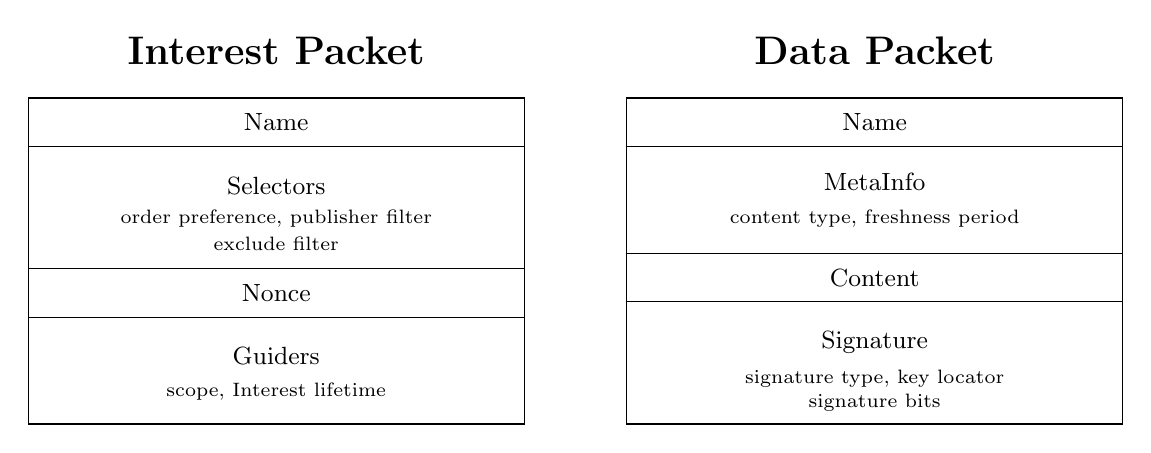
\begin{tikzpicture}[font=\small, every node/.style={align=center}]
\def\w{6.3}
\def\xA{-6.6}
\def\xB{1.0}
\node[font=\Large\bfseries] at (-3.45,2.95) {Interest Packet};
\draw (\xA,2.35) rectangle ++(\w,-0.62);
\node at (-3.45,2.04) {Name};
\draw (\xA,1.73) rectangle ++(\w,-1.55);
\node at (-3.45,1.24) {Selectors};
\node[font=\scriptsize] at (-3.45,0.82) {order preference, publisher filter};
\node[font=\scriptsize] at (-3.45,0.50) {exclude filter};
\draw (\xA,0.18) rectangle ++(\w,-0.62);
\node at (-3.45,-0.13) {Nonce};
\draw (\xA,-0.44) rectangle ++(\w,-1.35);
\node at (-3.45,-0.92) {Guiders};
\node[font=\scriptsize] at (-3.45,-1.38) {scope, Interest lifetime};

\node[font=\Large\bfseries] at (4.15,2.95) {Data Packet};
\draw (\xB,2.35) rectangle ++(\w,-0.62);
\node at (4.15,2.04) {Name};
\draw (\xB,1.73) rectangle ++(\w,-1.35);
\node at (4.15,1.28) {MetaInfo};
\node[font=\scriptsize] at (4.15,0.82) {content type, freshness period};
\draw (\xB,0.38) rectangle ++(\w,-0.62);
\node at (4.15,0.07) {Content};
\draw (\xB,-0.24) rectangle ++(\w,-1.55);
\node at (4.15,-0.76) {Signature};
\node[font=\scriptsize] at (4.15,-1.22) {signature type, key locator};
\node[font=\scriptsize] at (4.15,-1.52) {signature bits};
\end{tikzpicture}%
}
\caption{NDN Interest 和 Data packet 结构的简化图，根据 NDN 架构论文~\cite{ndn}重新绘制。}
\label{fig:ndn-packets-ch}
\end{figure}

接收端驱动获取和网内缓存很有用，但服务调用不只是获取单个对象。多个
provider 需要发现某个 request 已经发布，user 需要先收集 ACK metadata 再
选择 provider，长时间运行的任务还需要状态诊断。因此，NDNSF 使用 NDN
Sync，尤其是 NDN-SVS 实现的 State Vector Sync，让 user 和 provider 发现
新发布的服务消息，而不需要把服务绑定到固定端点
~\cite{li2018brief,moll2022sok,ndnsvs-github}。在 NDNSF 中，Sync 不是服
务语义本身，而是 Request、ACK、Selection 和 Response 等命名 Data 消息的
发布和发现底座。

实现层面，NDNSF 构建在标准 NDN 软件栈上。NFD 提供本地 forwarder 和 Face
抽象，\texttt{ndn-cxx} 提供 C++ 应用开发所需的名字、packet、Face、签名、
验证和 segmented object retrieval~\cite{ndn-cxx}。这些库使 NDNSF 可以使
用普通 NDN 名字和 packet，而不需要重新发明一套传输格式；同时也支持应用
通过 reference 传递大 artifact：模型、视频录制、图片、日志和中间推理数
据可以被分段成命名 Data packet，被签名、可选加密、按名字获取，并在小型
service-request payload 之外独立验证。

访问控制方面，NDNSF 使用 NAC-ABE，将 NDN 命名和属性基加密结合起来，使
服务级授权可以围绕名字表达，而不是围绕传输连接表达~\cite{dulal2023nacabe}。
NDNSF 将这一能力与 controller 分发的权限、服务级属性和每次调用的一次性
token 结合起来。由此，NDN 提供数据中心通信底座，而 NDNSF 提供服务层
runtime：谁可以调用服务、谁可以提供服务、如何选择 provider、如何保护消
息，以及如何把大型命名对象附加到服务 workflow 中。

\begin{table}[H]
\centering
\caption{NDN 基础组件如何对应 NDNSF 机制。}
\label{tab:ndn-to-ndnsf-ch}
\begin{tabularx}{\textwidth}{p{0.30\textwidth}X}
\toprule
NDN 基础组件 & NDNSF 机制 \\
\midrule
Data packet & Request、ACK、Selection 和 Response 是承载在命名 Data 中
的服务消息对象。 \\
Interest & Interest 用于按名字获取 Data；NDN-SVS 使用 Sync Interest 宣告
数据集更新。 \\
Data 签名和基于名字的 trust & service message、permission 和大对象可以独
立于返回路径或缓存位置被验证。 \\
FIB/PIT/CS 转发与缓存 & 服务相关数据可以按名字获取，并在移动、缓存和间
歇连接场景下保持语义。 \\
NDN Sync / SVS & user 和 provider 可以发现新发布的服务事件，而不需要把
服务绑定到固定 endpoint。 \\
分段 Data 获取 & 大模型、视频、日志和中间 tensor 通过 reference 携带，而
不是塞进小型 service payload。 \\
NAC-ABE 和命名属性 & 服务级权限和保密策略围绕名字与属性表达，而不是围
绕传输信道表达。 \\
\bottomrule
\end{tabularx}
\end{table}

\section{研究缺口}

因此，本文关注的研究缺口存在于 NDN 通信 primitives 和面向服务应用语义之
间。NDN 提供命名 Data、签名、缓存、转发状态、分段获取和基于 Sync 的发
现；但它本身并不定义 user 如何调用命名服务、授权 provider 如何发布
readiness、ACK metadata 如何收集、一个或多个 provider 如何被选择、replay
如何防止，以及大对象如何附着到服务 workflow。NDNSF 将这些功能上升为可复
用 framework mechanisms，而不是让每个应用各自拼接 glue code。

\section{论文论点}

本论文认为，动态面向服务应用和主机中心服务框架之间存在反复出现的不匹配：
应用希望围绕命名服务、命名能力、命名数据和可验证结果组织逻辑，而底层网
络栈通常暴露的是地址、信道和端点。数据中心服务框架可以通过在 NDN 名字
和可验证 Data packet 之上显式提供服务调用、授权、服务提供者选择、协作和
大对象获取抽象，缓解这种不匹配。

NDNSF v0.1 是本博士论文已经完成的核心贡献之一，并证明这一方向具有可行
性。后续博士论文工作将在这一基础上，将 NDNSF 扩展成面向真实动态服务应
用的框架，并通过两个高压力应用领域验证其设计：

\begin{itemize}
  \item \textbf{UAV 网络应用}代表移动、命令敏感、实时的 service-container
  workload。这类应用同时涉及间歇连接、命令授权、遥测、实时视频、录制、
  目标检测和多无人机任务协作。
  \item \textbf{分布式 AI 推理应用}代表 artifact 密集、多阶段的计算/数据
  协作 workload。这类应用需要在多个服务提供者之间协调模型分片、运行时
  artifact、中间张量、大数据对象和协作计划。
\end{itemize}

论文的核心命题是：如果服务、数据、权限和协作计划都可以被命名和验证，
那么应用就可以在动态环境中更自然地发现服务、选择提供者、保护数据并从故
障中恢复。

\section{研究问题}

\begin{enumerate}[label=RQ\arabic*., leftmargin=*]
  \item 主机中心服务框架在移动性、服务发现、安全验证和数据获取方面会产
  生哪些结构性问题？其中哪些可以通过数据中心服务命名和可验证 Data 得到
  缓解？
  \item NDNSF 应如何把服务调用、授权、服务提供者选择、协作和大对象获取
  抽象成通用 framework 机制，而不是让每个应用重新设计一个专用 NDN 协议？
  \item 当 NDN 服务请求可以发布给多个服务提供者，并通过 ACK metadata、
  provider selection 和 provider collaboration 解析时，会产生哪些可靠性、安
  全性和延迟 tradeoff？Targeted invocation 和 compensation 等支撑机制应如
  何使用？
  \item UAV 网络应用如何在移动、命令敏感、实时 service-container 场景下
  评估 NDNSF？
  \item 分布式 AI 推理如何在 artifact 密集、多阶段、计算/数据协作场景下
  评估 NDNSF？
\end{enumerate}

\subsection{预期回答形式}

本文预期以如下形式回答这些问题。RQ1 应识别一组反复出现的服务应用问题：
这些问题不只是已有系统的工程实现缺口，而是服务被绑定到 host、session 或
channel 后产生的结构性后果。RQ2 应说明 NDNSF 可以把服务调用、授权、
provider selection 和 provider collaboration 暴露为可复用框架机制；本地组
合和大数据引用则作为支撑性抽象，避免每个应用重新设计专用 NDN 协议。RQ3 应刻画 one-to-many request
publication、ACK metadata、provider selection 和 provider collaboration 在
什么情况下能改善可靠性，以及 Targeted invocation 或 compensation 等支撑
机制何时用于控制延迟和恢复成本，同时不削弱安全检查。RQ4 应说明 UAV
workload 如何在移动性、命令敏感性、实时视频和多无人机协作压力下检验同
一组框架机制。RQ5 应说明分布式推理如何在 artifact provisioning、tensor
dependency exchange、provider role assignment 和长时间分布式执行压力下
检验同一组机制。

\section{预期贡献}

本文预期贡献如下：

\begin{enumerate}[leftmargin=*]
  \item 一个面向 NDN 的通用、安全、动态服务框架 NDNSF。
  \item 以服务提供者协作为核心的 NDNSF 扩展，并包含 Targeted invocation、
  trusted local service composition 和大数据引用等支撑机制。
  \item 一个基于 NDNSF 的 UAV service-container 应用，覆盖飞控、遥测、
  视频、加密录制、目标检测和协作巡逻服务。
  \item 一个基于 NDNSF 的分布式 AI 推理应用，覆盖模型切分、服务计划、
  基于 reference 的 artifact exchange 和自动协作计划生成。
  \item 使用 MiniNDN、SITL UAV 实验和部分真机验证对 NDNSF 及应用原型进
  行评估。
\end{enumerate}

\section{Proposal 范围边界}

为保持 proposal 的边界清晰，本文将 NDNSF v0.1 视为博士论文已经完成的核
心基础成果，而不是最终完整系统。NDNSF v0.1 已经建立了 data-centric
service framework 的基本架构，并证明了这一方向的可行性。后续博士论文工
作将在这一基础上，把 NDNSF 扩展成经过应用验证的 framework。主要框架扩
展是 provider collaboration：多个已授权 provider 如何发现 request、发布能
力或状态、被选择、交换状态或 artifact，并共同完成一个服务任务。Targeted
invocation、trusted local invocation 和 large-data reference 是让这一协作服务
模型在低延迟调用、同进程组合和大对象 workload 中可落地的支撑机制。这些
机制不是 UAV 专用或 AI 专用功能，而是拟作为 NDNSF 通用机制完成并评估的
设计。

因此，本论文的核心问题不是能否实现两个应用，而是 NDNSF 是否能够提供可
复用的数据中心服务机制，并且这些机制能否在两个差异很大的 workload 中保
持成立。

UAV 应用用于验证 NDNSF 是否适合作为移动、命令敏感、实时系统的
service-container framework。它的设计会检验结构化遥测、任务、视频和安
全信息、Targeted 飞控命令、自适应直播视频、加密本地录制、目标检测服务
组合和多无人机协作巡逻。DistributedInference 应用用于验证 NDNSF 是
否适合作为 artifact 密集、多阶段计算/数据协作的 framework。它的设计会检
验自动模型计划生成、基于 reference 的模型和 activation artifact、可预测可预取
对象名称，以及基于 tensor DAG 的依赖驱动执行。也就是说，UAV 和
DistributedInference 不是两个孤立 demo，而是用于验证同一个 data-centric
service framework thesis 的两个互补压力场景。

这两个应用也会反向提出 NDNSF 的框架需求。UAV workload 会压力测试低延
迟命令调用、结构化命令状态、service-container 组合和视频大数据引用；
DistributedInference workload 会压力测试依赖驱动协作、artifact reference、
provider role assignment 和长任务 selection 诊断。因此，应用工作在论文中
有双重意义：它们本身是有价值的应用系统，同时也是验证和完善 provider
collaboration 这一核心 NDNSF 扩展的主要方法。
